% ============================================================================
%  Erdos Problem 915 -- thesis defence slides
%  Louis Vandenbruwaene, KU Leuven, Master of Mathematics
%
%  Build:  cd slides && latexmk -pdf slides.tex   (or pdflatex twice)
%  Reuses the thesis house style from ../shared/colors.tex and tikz-styles.tex.
% ============================================================================
\documentclass[aspectratio=169,11pt]{beamer}

\usepackage[T1]{fontenc}
\usepackage[utf8]{inputenc}
\usepackage{helvet}
\renewcommand{\familydefault}{\sfdefault}
\usepackage{amsmath,amssymb}
\usepackage{booktabs}
\usepackage{graphicx}
\usepackage{tikz}
\usetikzlibrary{calc,arrows.meta,shapes.geometric,positioning,
                decorations.pathmorphing,backgrounds,fit,shadows,patterns}

% ---- thesis colours and graph styles (reused, single source of truth) -------
% ============================================================================
% UNIFIED COLOR DEFINITIONS FOR ERDOS PROBLEM 915 THESIS
% ============================================================================
% This file provides consistent colors across thesis, progress report, and
% presentation. All colors are based on KU Leuven institutional branding.
% ============================================================================

% --- KU Leuven Primary Colors ---
% Note: In beamer (kulakbeamer), KULblauw1/KULblauw3a/KULblauw3b are predefined
% For thesis documents, we define them here
\makeatletter
\@ifclassloaded{kulakbeamer}{%
    % Colors already defined by beamer class
}{%
    % Define KUL colors for non-beamer documents
    \definecolor{KULblauw1}{RGB}{29,141,176}     % Main blue
    \definecolor{KULblauw3a}{RGB}{82,189,236}    % Accent light blue
    \definecolor{KULblauw3b}{RGB}{30,110,135}    % Accent dark blue
}
\makeatother

% --- Graph Vertex Colors ---
% Primary vertex color uses KUL blue
\definecolor{vertexblue}{RGB}{29,141,176}        % KULblauw1
\definecolor{vertexred}{RGB}{200,80,80}          % Matched with presentation
\definecolor{vertexpurple}{RGB}{140,80,160}      % Matched with presentation
\definecolor{vertexgreen}{RGB}{60,160,80}        % Matched with presentation
\definecolor{vertexorange}{RGB}{220,140,40}      % Matched with presentation

% --- Aliases for presentation compatibility ---
\colorlet{graphred}{vertexred}
\colorlet{graphpurple}{vertexpurple}
\colorlet{graphgreen}{vertexgreen}
\colorlet{graphorange}{vertexorange}

% ============================================================================
% UNIFIED TIKZ STYLES FOR ERDOS PROBLEM 915 THESIS
% ============================================================================
% This file provides consistent TikZ graph styles across thesis, progress
% report, and presentation. Requires colors.tex to be loaded first.
% ============================================================================

% --- Vertex Styles ---
\tikzset{
    % Basic vertex style (KUL blue)
    vertex/.style={
        circle, draw=KULblauw1, fill=KULblauw1!15,
        minimum size=20pt, inner sep=0pt,
        font=\small\bfseries, line width=1.5pt
    },
    % Small vertex for complex diagrams
    smallvertex/.style={
        circle, draw=KULblauw1, fill=KULblauw1!15,
        minimum size=16pt, inner sep=0pt,
        font=\scriptsize\bfseries, line width=1.2pt
    },
    % Colored variants - semantic naming
    leftvertex/.style={vertex, draw=KULblauw1, fill=KULblauw1!15},
    rightvertex/.style={vertex, draw=vertexred, fill=vertexred!15},
    sharedvertex/.style={vertex, draw=vertexpurple, fill=vertexpurple!20},
    tailvertex/.style={vertex, draw=vertexgreen, fill=vertexgreen!15},
    hubvertex/.style={vertex, draw=vertexorange, fill=vertexorange!20},
    % Small colored variants
    smallleftvertex/.style={smallvertex, draw=KULblauw1, fill=KULblauw1!15},
    smallrightvertex/.style={smallvertex, draw=vertexred, fill=vertexred!15},
    smallsharedvertex/.style={smallvertex, draw=vertexpurple, fill=vertexpurple!20},
    smalltailvertex/.style={smallvertex, draw=vertexgreen, fill=vertexgreen!15},
    % Presentation-style aliases (gnode = graph node)
    gnode/.style={vertex},
    bluenode/.style={leftvertex},
    rednode/.style={rightvertex},
    purplenode/.style={sharedvertex},
    greennode/.style={tailvertex},
    orangenode/.style={hubvertex},
}

% --- Edge Styles ---
\tikzset{
    % Basic edge styles
    edge/.style={line width=1.8pt, KULblauw1!70},
    thickedge/.style={line width=2.5pt},
    % Colored edge variants - semantic naming
    leftedge/.style={line width=1.8pt, KULblauw1},
    rightedge/.style={line width=1.8pt, vertexred},
    sharededge/.style={line width=1.8pt, vertexpurple!80},
    tailedge/.style={line width=1.8pt, vertexgreen!80!black},
    % Tree edges
    treeedge/.style={line width=1.8pt, KULblauw3b},
    lefttreeedge/.style={line width=1.8pt, KULblauw1},
    righttreeedge/.style={line width=1.8pt, vertexred},
    % Special edge styles
    missingedge/.style={line width=1.5pt, dashed, gray},
    multiedge/.style={line width=1.5pt, draw=KULblauw3b},
    hyperedge/.style={draw=vertexred, fill=vertexred!10, rounded corners=8pt, line width=1.5pt},
    % Presentation-style aliases
    gedge/.style={line width=2pt, KULblauw1!70},
    blueedge/.style={line width=2pt, KULblauw1},
    rededge/.style={line width=2pt, vertexred},
    purpleedge/.style={line width=2pt, vertexpurple!80},
    greenedge/.style={line width=2pt, vertexgreen!80!black},
    tedge/.style={treeedge},
}

% --- Directed arc styles (Stealth arrowheads, thesis blue) ---
% A global `arc` is safe: figures that set their own `arc/.style` inline
% (e.g. the Chapter 1 hub figures) shadow this within their own picture.
\tikzset{
    arc/.style={-{Stealth[length=2.2mm]}, line width=1.1pt, KULblauw1},
    faintarc/.style={-{Stealth[length=1.8mm]}, line width=0.7pt, KULblauw1!35},
    redarc/.style={-{Stealth[length=2.2mm]}, line width=1.1pt, dashed, vertexred},
    forbiddenedge/.style={line width=1.3pt, dashed, vertexred},
}

% --- Hyperedge node: a hollow square standing for a hyperedge (e.g. in an
%     incidence graph), distinct from the `hyperedge` region style above ---
\tikzset{
    hnode/.style={
        rectangle, draw=KULblauw3b, fill=white,
        minimum size=13pt, inner sep=1pt, line width=1pt,
        font=\scriptsize\bfseries
    },
}

% --- Label and Weight Styles ---
\tikzset{
    treeweight/.style={
        circle, fill=white, inner sep=1.5pt,
        font=\scriptsize\bfseries
    },
    tweight/.style={
        circle, fill=white, inner sep=2pt,
        font=\small\bfseries
    },
    edgelabel/.style={
        font=\scriptsize, fill=white, inner sep=1pt
    }
}

\graphicspath{{../figures/}{../}}

% ---- semantic status colours (used on the landscape table and the ladder) ---
\colorlet{stProved}{vertexgreen!75!black}
\colorlet{stMachine}{KULblauw1}
\colorlet{stConj}{vertexorange!90!black}
\colorlet{stOpen}{vertexred}

% ---- small helpers ----------------------------------------------------------
\newcommand{\Erdos}{Erd\H{o}s}
\newcommand{\floor}[1]{\left\lfloor #1\right\rfloor}
\newcommand{\lmax}{\lambda^{\max}}
\newcommand{\kmax}{\kappa^{\max}}
\newcommand{\chip}[2]{\tikz[baseline=-0.55ex]{\node[rounded corners=2pt,
   fill=#1,text=white,inner xsep=4pt,inner ysep=2pt,
   font=\scriptsize\bfseries]{#2};}}

% ============================================================================
%  THEME
% ============================================================================
\setbeamertemplate{navigation symbols}{}
\usefonttheme{professionalfonts}

\setbeamercolor{structure}{fg=KULblauw1}
\setbeamercolor{frametitle}{fg=KULblauw3b}
\setbeamercolor{title}{fg=KULblauw3b}
\setbeamercolor{normal text}{fg=black!88}
\setbeamercolor{itemize item}{fg=KULblauw1}
\setbeamercolor{itemize subitem}{fg=KULblauw3a}
\setbeamerfont{frametitle}{series=\bfseries,size=\Large}
\setbeamerfont{title}{series=\bfseries}
\setbeamertemplate{itemize item}{\small\raise0.5pt\hbox{\textbullet}}
\setbeamertemplate{itemize subitem}{\scriptsize\raise0.5pt\hbox{\textendash}}

% frame title with a thin accent rule beneath
\setbeamertemplate{frametitle}{%
  \vskip4pt%
  \begin{beamercolorbox}[wd=\paperwidth,leftskip=0.9cm,rightskip=0.9cm]{frametitle}%
    \usebeamerfont{frametitle}\insertframetitle%
  \end{beamercolorbox}%
  \vskip2pt%
  \hspace*{0.9cm}{\color{KULblauw3a}\rule{0.82\paperwidth}{1.3pt}}%
  \vskip2pt%
}

% slim footline: short title (left) and frame number (right)
\setbeamertemplate{footline}{%
  \hbox{%
    \begin{beamercolorbox}[wd=0.72\paperwidth,ht=2.4ex,dp=1.2ex,leftskip=0.9cm]{}%
      {\scriptsize\color{black!45}\Erdos{} Problem 915}%
    \end{beamercolorbox}%
    \begin{beamercolorbox}[wd=0.28\paperwidth,ht=2.4ex,dp=1.2ex,rightskip=0.9cm]{}%
      \hfill{\scriptsize\color{black!45}\insertframenumber\,/\,\inserttotalframenumber}%
    \end{beamercolorbox}%
  }%
}

\setbeamersize{text margin left=0.9cm,text margin right=0.9cm}

% ============================================================================
\begin{document}

% ----------------------------------------------------------------------------
% S1  TITLE
% ----------------------------------------------------------------------------
\begin{frame}[plain]
\begin{tikzpicture}[remember picture,overlay]
  % faint decorative graph, top right
  \begin{scope}[shift={($(current page.north east)+(-2.7,-2.0)$)},scale=0.9,opacity=0.18]
    \foreach \i in {0,...,6}{\coordinate (d\i) at ({51.43*\i}:1.4);}
    \foreach \i in {0,...,6}{\foreach \j in {0,...,6}{\draw[KULblauw1,line width=0.7pt] (d\i)--(d\j);}}
    \foreach \i in {0,...,6}{\fill[KULblauw3b] (d\i) circle (2.6pt);}
  \end{scope}
  % accent bar
  \fill[KULblauw1] ($(current page.west)+(0,1.55)$) rectangle ($(current page.east)+(0,1.49)$);
  \fill[KULblauw3a] ($(current page.west)+(0,1.49)$) rectangle ($(current page.east)+(0,1.46)$);
\end{tikzpicture}

\vspace{1.7cm}
\hspace*{0.4cm}\begin{minipage}{0.92\textwidth}
  {\color{black!40}\large EXTREMAL GRAPH THEORY}\\[10pt]
  {\color{KULblauw3b}\fontsize{38}{42}\selectfont\bfseries \Erdos{} Problem 915}\\[8pt]
  {\color{KULblauw1}\Large From Proof to Search}\\[4pt]
  {\color{black!70}\large One extremal question, carried across twelve variants.}

  \vspace{1.5cm}
  {\large\bfseries Louis Vandenbruwaene}\\[3pt]
  {\small\color{black!70}Supervisor: Prof.\ Stijn Cambie \qquad Promotor: Prof.\ Jan Goedgebeur}\\[2pt]
  {\small\color{black!70}KU Leuven, Faculty of Science, Master of Mathematics}
\end{minipage}

\begin{tikzpicture}[remember picture,overlay]
  \node[anchor=south east] at ($(current page.south east)+(-0.8,0.5)$)
    {
\includegraphics[height=1.0cm]{LogoKULeuven.png}};
\end{tikzpicture}
\end{frame}

% ----------------------------------------------------------------------------
% S2  THE WALL METAPHOR
% ----------------------------------------------------------------------------
\begin{frame}{A hard problem is a wall}
\centering
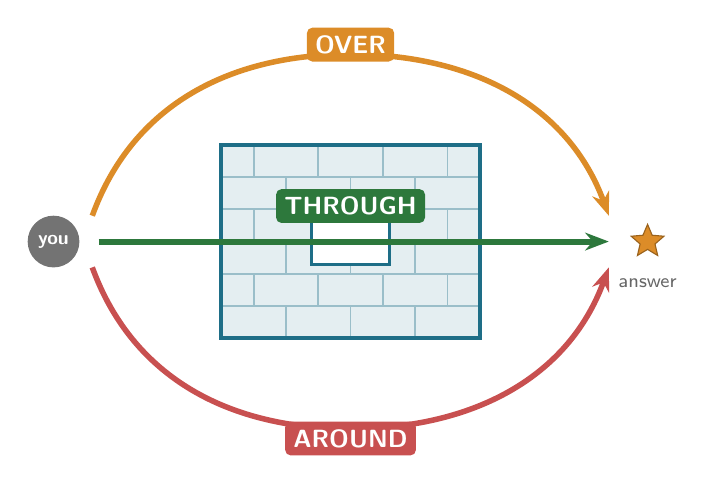
\begin{tikzpicture}[scale=0.82]
  % --- the wall ---
  \begin{scope}
    \fill[KULblauw3b!12] (0,0) rectangle (4,3);
    % mortar rows
    \foreach \y in {0.5,1.0,1.5,2.0,2.5}{\draw[KULblauw3b!45,line width=0.6pt] (0,\y)--(4,\y);}
    % staggered bricks
    \foreach \y in {0,1.0,2.0}{\foreach \x in {1,2,3}{\draw[KULblauw3b!45,line width=0.6pt] (\x,\y)--(\x,\y+0.5);}}
    \foreach \y in {0.5,1.5,2.5}{\foreach \x in {0.5,1.5,2.5,3.5}{\draw[KULblauw3b!45,line width=0.6pt] (\x,\y)--(\x,\y+0.5);}}
    \draw[KULblauw3b,line width=1.4pt] (0,0) rectangle (4,3);
  \end{scope}

  % start and goal markers
  \node[circle,fill=black!55,text=white,font=\scriptsize\bfseries,inner sep=2.5pt] (S) at (-2.6,1.5) {you};
  \node[star,star points=5,star point ratio=2.2,fill=vertexorange,draw=vertexorange!70!black,
        inner sep=2pt] (G) at (6.6,1.5) {};
  \node[font=\scriptsize\color{black!60}] at (6.6,0.85) {answer};

  % OVER  (over the top)
  \draw[line width=2pt,vertexorange,-{Stealth[length=3mm]}]
        (-2.0,1.9) to[out=70,in=180] (2,4.4) to[out=0,in=110] (6.0,1.9);
  \node[fill=vertexorange,text=white,rounded corners=2pt,font=\bfseries\small,inner sep=3pt]
        at (2,4.55) {OVER};

  % THROUGH (straight through a gap)
  \fill[white] (1.4,1.15) rectangle (2.6,1.85);
  \draw[KULblauw3b,line width=1pt] (1.4,1.15) rectangle (2.6,1.85);
  \draw[line width=2.2pt,vertexgreen!75!black,-{Stealth[length=3mm]}] (-1.9,1.5)--(6.0,1.5);
  \node[fill=vertexgreen!75!black,text=white,rounded corners=2pt,font=\bfseries\small,inner sep=3pt]
        at (2,2.05) {THROUGH};

  % AROUND (around the bottom)
  \draw[line width=2pt,vertexred,-{Stealth[length=3mm]}]
        (-2.0,1.1) to[out=-70,in=180] (2,-1.4) to[out=0,in=250] (6.0,1.1);
  \node[fill=vertexred,text=white,rounded corners=2pt,font=\bfseries\small,inner sep=3pt]
        at (2,-1.55) {AROUND};
\end{tikzpicture}

\vspace{0.1cm}
{\color{black!75}\large Facing an obstacle, there are three ways past it. Mathematics has the same three.}
\end{frame}

% ----------------------------------------------------------------------------
% S3  THREE WAYS IN MATH
% ----------------------------------------------------------------------------
\begin{frame}{Three ways past the wall}
\small
The ``best solution'' of an extremal problem is the densest graph allowed by the rule. Three routes reach it.

\vspace{0.4cm}
\begin{columns}[t,onlytextwidth]
  \begin{column}{0.32\textwidth}\centering
    
\begin{tikzpicture}\node[draw=vertexgreen!75!black,line width=1.4pt,rounded corners=4pt,
        fill=vertexgreen!8,minimum width=3.4cm,minimum height=1.0cm,
        font=\bfseries,text=vertexgreen!55!black]{THROUGH};\end{tikzpicture}\\[6pt]
    {\bfseries Proof}\\[3pt]
    A single clean argument that settles every $n$ at once.\\[4pt]
    {\scriptsize\color{black!55}Mader, Menger, Gomory-Hu, a hand induction.}
  \end{column}
  \begin{column}{0.32\textwidth}\centering
    
\begin{tikzpicture}\node[draw=vertexorange!85!black,line width=1.4pt,rounded corners=4pt,
        fill=vertexorange!10,minimum width=3.4cm,minimum height=1.0cm,
        font=\bfseries,text=vertexorange!60!black]{OVER};\end{tikzpicture}\\[6pt]
    {\bfseries Calculation}\\[3pt]
    Check a finite domain exactly, by machine, and emit a certificate.\\[4pt]
    {\scriptsize\color{black!55}Exact max-flow, cut-counting upper bounds.}
  \end{column}
  \begin{column}{0.32\textwidth}\centering
    
\begin{tikzpicture}\node[draw=vertexred,line width=1.4pt,rounded corners=4pt,
        fill=vertexred!8,minimum width=3.4cm,minimum height=1.0cm,
        font=\bfseries,text=vertexred!75!black]{AROUND};\end{tikzpicture}\\[6pt]
    {\bfseries Approximation}\\[3pt]
    Search for good examples. Gives lower bounds, never the front door.\\[4pt]
    {\scriptsize\color{black!55}Simulated annealing, tabu search.}
  \end{column}
\end{columns}

\vspace{0.5cm}
\begin{center}\itshape\color{KULblauw3b}
This thesis uses all three, and is honest about which one each answer rests on.
\end{center}
\end{frame}

% ----------------------------------------------------------------------------
% S4  THE ROAD OF A PROBLEM
% ----------------------------------------------------------------------------
\begin{frame}{The road of a research problem}
\centering
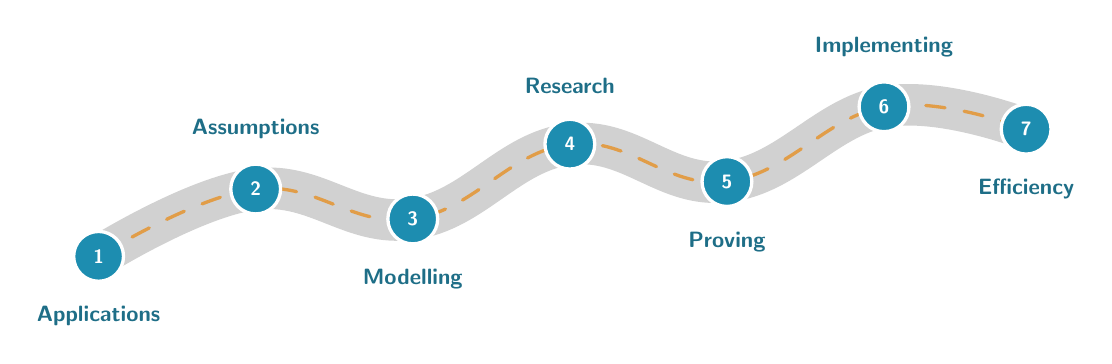
\begin{tikzpicture}[scale=0.95,
   stop/.style={circle,fill=KULblauw1,text=white,font=\scriptsize\bfseries,
                inner sep=0pt,minimum size=18pt,draw=white,line width=1.2pt},
   lab/.style={font=\footnotesize\bfseries,text=KULblauw3b}]
  % the road
  \draw[line width=15pt,black!18,line cap=round]
     plot[smooth,tension=0.7] coordinates {(0,0)(2.1,0.9)(4.2,0.5)(6.3,1.5)(8.4,1.0)(10.5,2.0)(12.4,1.7)};
  \draw[line width=1.2pt,vertexorange!85,dash pattern=on 7pt off 7pt,line cap=round]
     plot[smooth,tension=0.7] coordinates {(0,0)(2.1,0.9)(4.2,0.5)(6.3,1.5)(8.4,1.0)(10.5,2.0)(12.4,1.7)};

  % milestones (alternating labels above/below)
  \node[stop] (m1) at (0,0)    {1}; \node[lab,below=5pt of m1]      {Applications};
  \node[stop] (m2) at (2.1,0.9){2}; \node[lab,above=5pt of m2]      {Assumptions};
  \node[stop] (m3) at (4.2,0.5){3}; \node[lab,below=5pt of m3]      {Modelling};
  \node[stop] (m4) at (6.3,1.5){4}; \node[lab,above=5pt of m4]      {Research};
  \node[stop] (m5) at (8.4,1.0){5}; \node[lab,below=5pt of m5]      {Proving};
  \node[stop] (m6) at (10.5,2.0){6};\node[lab,above=5pt of m6]      {Implementing};
  \node[stop] (m7) at (12.4,1.7){7};\node[lab,below=5pt of m7]      {Efficiency};
\end{tikzpicture}

\vspace{0.6cm}
{\color{black!75}\large Every problem travels this road. The slides ahead follow it, from the rule
to the running code.}
\end{frame}

% ----------------------------------------------------------------------------
% S5  THE PROBLEM, PRECISELY
% ----------------------------------------------------------------------------
\begin{frame}{Problem 915, precisely}
\begin{columns}[c,onlytextwidth]
  \begin{column}{0.42\textwidth}\centering
    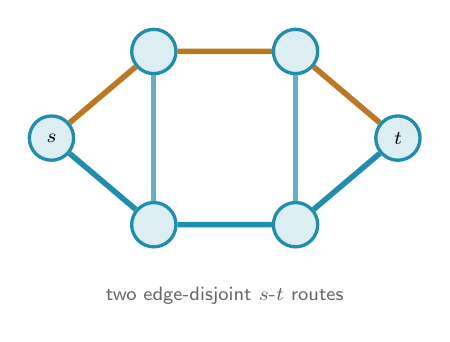
\begin{tikzpicture}[scale=1.0,every node/.style={transform shape}]
      \node[smallvertex] (s) at (-2.2,0)   {$s$};
      \node[smallvertex] (a) at (-0.9,1.1) {};
      \node[smallvertex] (b) at (0.9,1.1)  {};
      \node[smallvertex] (c) at (-0.9,-1.1){};
      \node[smallvertex] (d) at (0.9,-1.1) {};
      \node[smallvertex] (t) at (2.2,0)    {$t$};
      % two edge-disjoint s-t routes
      \draw[line width=2pt,vertexorange!85!black] (s)--(a)--(b)--(t);
      \draw[line width=2pt,KULblauw1] (s)--(c)--(d)--(t);
      % extra edges to make it a real graph
      \draw[edge] (a)--(c); \draw[edge] (b)--(d);
      \node[font=\scriptsize\color{black!60}] at (0,-2.0) {two edge-disjoint $s$-$t$ routes};
    \end{tikzpicture}
  \end{column}
  \begin{column}{0.55\textwidth}\small
    A graph $G$: $n$ vertices, $E$ edges.\\[3pt]
    {\bfseries Independent routes.} $\lambda_G(u,v)$ is the largest number of edge-disjoint
    $u$-$v$ paths. By Menger, also the cheapest cut between them.\\[3pt]
    {\bfseries Binding connectivity.}
    \[\lmax_G=\max_{u,v}\lambda_G(u,v).\]
    {\bfseries The rule.} No pair gets $m$ routes: \;$\lmax_G\le m-1$.\\[3pt]
    {\bfseries The goal.} Pack in as many edges as the rule allows:
    \[\ell_m(n)=\max\{\,|E|:\lmax_G\le m-1\,\}.\]
  \end{column}
\end{columns}

\vspace{0.05cm}
\begin{center}
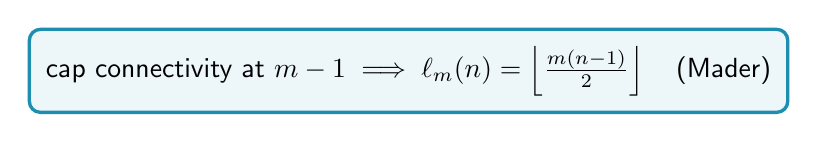
\begin{tikzpicture}
  \node[draw=KULblauw1,line width=1.2pt,rounded corners=4pt,fill=KULblauw1!8,
        inner sep=6pt]{$\displaystyle \text{cap connectivity at } m-1 \;\Longrightarrow\;
        \ell_m(n)=\floor{\tfrac{m(n-1)}{2}} \quad\text{(Mader)}$};
\end{tikzpicture}
\end{center}
\end{frame}

% ----------------------------------------------------------------------------
% S6  APPLICATIONS
% ----------------------------------------------------------------------------
\begin{frame}{What is it good for?}
\small
{\large\color{KULblauw3b}\bfseries Honest answer: no direct application.}
\;But in mathematics the road often matters more than the destination.

\vspace{0.5cm}
\begin{columns}[t,onlytextwidth]
  \begin{column}{0.32\textwidth}
    {\bfseries\color{KULblauw1}The question}\\[4pt]
    How do you quantify the redundancy of a network: the spare, independent routes
    it keeps between its points? Graphs turn that into a vast space to search.
  \end{column}
  \begin{column}{0.32\textwidth}
    {\bfseries\color{KULblauw1}The transferable tools}\\[4pt]
    \begin{itemize}\itemsep2pt
      \item maximum-flow connectivity
      \item temperature-guided search
      \item machine-checked certificates
    \end{itemize}
  \end{column}
  \begin{column}{0.32\textwidth}
    {\bfseries\color{KULblauw1}Where redundancy lives}\\[4pt]
    \begin{itemize}\itemsep2pt
      \item electricity grids
      \item pipelines
      \item road and rail networks
    \end{itemize}
    \vspace{2pt}{\scriptsize\color{black!55}Backup routes everywhere.}
  \end{column}
\end{columns}

\vspace{0.55cm}
\begin{center}\itshape\color{black!70}
The methods outlive the single number they were built to find.
\end{center}
\end{frame}

% ----------------------------------------------------------------------------
% S7  TWELVE VARIANTS
% ----------------------------------------------------------------------------
\begin{frame}{One question, twelve variants}
\small Change the rules of the network one axis at a time.

\vspace{0.45cm}
\centering
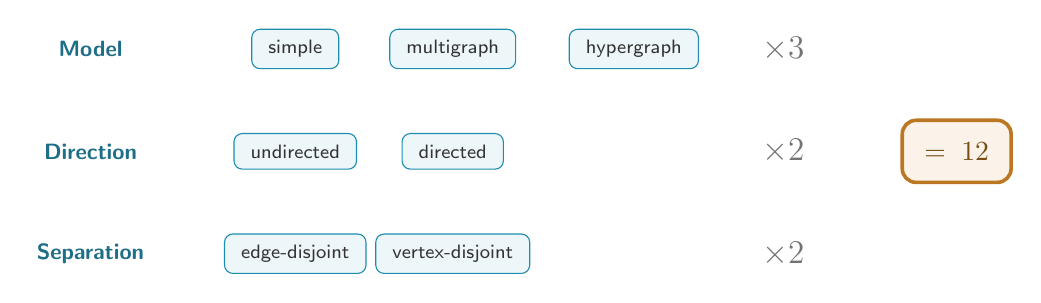
\begin{tikzpicture}[
   ax/.style={font=\footnotesize\bfseries,text=KULblauw3b},
   opt/.style={rounded corners=3pt,draw=KULblauw1,fill=KULblauw1!8,
               font=\scriptsize,inner xsep=6pt,inner ysep=4pt,text=black!80}]
  % axis 1: model
  \node[ax] at (-5.6,2) {Model};
  \node[opt] (md1) at (-3.0,2) {simple};
  \node[opt] (md2) at (-1.0,2) {multigraph};
  \node[opt] (md3) at (1.3,2)  {hypergraph};
  \node[font=\large\bfseries,text=black!55] at (3.2,2) {$\times 3$};

  % axis 2: direction
  \node[ax] at (-5.6,0.7) {Direction};
  \node[opt] (dr1) at (-3.0,0.7) {undirected};
  \node[opt] (dr2) at (-1.0,0.7) {directed};
  \node[font=\large\bfseries,text=black!55] at (3.2,0.7) {$\times 2$};

  % axis 3: separation
  \node[ax] at (-5.6,-0.6) {Separation};
  \node[opt] (sp1) at (-3.0,-0.6) {edge-disjoint};
  \node[opt] (sp2) at (-1.0,-0.6) {vertex-disjoint};
  \node[font=\large\bfseries,text=black!55] at (3.2,-0.6) {$\times 2$};

  % result
  \node[draw=vertexorange!85!black,line width=1.3pt,fill=vertexorange!10,rounded corners=5pt,
        font=\bfseries,text=vertexorange!55!black,inner sep=8pt] at (5.4,0.7) {$=\;12$};
\end{tikzpicture}

\vspace{0.45cm}
{\color{black!75}Mader's clean theorem is one corner. The other eleven are the journey, and they
get harder as the model gets richer.}
\end{frame}

% ----------------------------------------------------------------------------
% S8  k vs l
% ----------------------------------------------------------------------------
\begin{frame}{Edge routes versus vertex routes}
\begin{columns}[c,onlytextwidth]
  \begin{column}{0.56\textwidth}\centering
    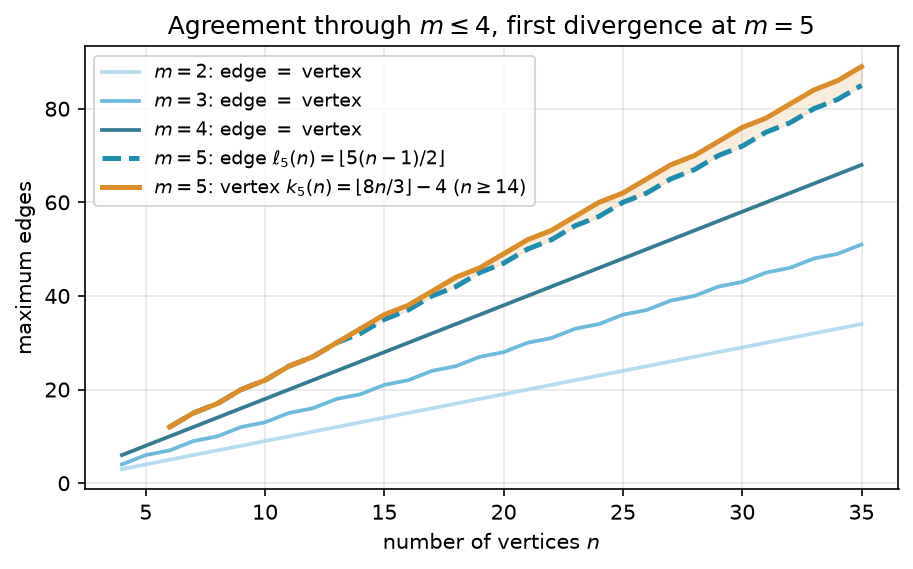
\includegraphics[width=\linewidth]{edge_vertex_divergence.png}
  \end{column}
  \begin{column}{0.42\textwidth}\small
    Two separations: routes may avoid sharing an {\bfseries edge} ($\lambda$) or, more strictly,
    an internal {\bfseries vertex} ($\kappa$). Whitney: $\kappa\le\lambda$.\\[8pt]
    \chip{stProved}{$m\le 4$}\; the two problems give the {\bfseries same} answer
    (Leonard).\\[8pt]
    \chip{stConj}{$m=5$}\; first divergence (S{\o}rensen-Thomassen):
    \[k_5(n)=\floor{\tfrac{8n}{3}}-3 \;>\; \ell_5(n).\]
    \chip{stOpen}{$m\ge 6$}\; open since 1974. The extremal structure is genuinely
    not understood. The one direction the thesis does not try to force.
  \end{column}
\end{columns}
\end{frame}

% ----------------------------------------------------------------------------
% S9  WHAT FELL AND HOW HARD
% ----------------------------------------------------------------------------
\begin{frame}{What fell, and how hard}
\small How each variant is known, from a clean argument to a stubborn blank.

\vspace{0.5cm}
\centering
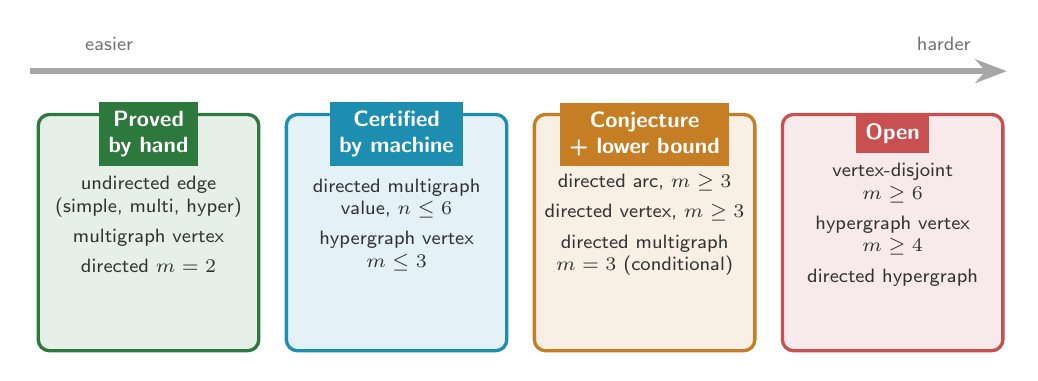
\begin{tikzpicture}[
   bin/.style={rounded corners=4pt,minimum width=2.8cm,minimum height=3.0cm,line width=1.2pt},
   hd/.style={font=\bfseries\footnotesize,text=white,align=center},
   it/.style={font=\scriptsize,align=center,text=black!80}]
  % gradient of difficulty arrow
  \draw[-{Stealth[length=4mm]},line width=2pt,black!35] (-6.2,2.05) -- (6.2,2.05);
  \node[font=\scriptsize\color{black!55}] at (-5.2,2.4) {easier};
  \node[font=\scriptsize\color{black!55}] at (5.4,2.4)  {harder};

  \node[bin,fill=stProved!12,draw=stProved] (b1) at (-4.7,0) {};
  \node[bin,fill=stMachine!12,draw=stMachine] (b2) at (-1.55,0) {};
  \node[bin,fill=stConj!12,draw=stConj] (b3) at (1.6,0) {};
  \node[bin,fill=stOpen!12,draw=stOpen] (b4) at (4.75,0) {};

  \node[hd,fill=stProved]  at (-4.7,1.25) {Proved\\by hand};
  \node[hd,fill=stMachine] at (-1.55,1.25){Certified\\by machine};
  \node[hd,fill=stConj]    at (1.6,1.25)  {Conjecture\\+ lower bound};
  \node[hd,fill=stOpen]    at (4.75,1.25) {Open};

  \node[it] at (-4.7,0.1) {undirected edge\\(simple, multi, hyper)\\[3pt]
                           multigraph vertex\\[3pt] directed $m=2$};
  \node[it] at (-1.55,0.1){directed multigraph\\value, $n\le 6$\\[3pt]
                           hypergraph vertex\\$m\le 3$};
  \node[it] at (1.6,0.1)  {directed arc, $m\ge 3$\\[3pt] directed vertex, $m\ge 3$\\[3pt]
                           directed multigraph\\$m=3$ (conditional)};
  \node[it] at (4.75,0.1) {vertex-disjoint\\$m\ge 6$\\[3pt]
                           hypergraph vertex\\$m\ge 4$\\[3pt] directed hypergraph};
\end{tikzpicture}

\vspace{0.35cm}
{\scriptsize\color{black!60}The honesty contract: search proves nothing on its own. A value is
``settled'' only with a matching hand proof or a machine certificate.}
\end{frame}

% ----------------------------------------------------------------------------
% S10  HOW THE MACHINE WORKS
% ----------------------------------------------------------------------------
\begin{frame}{How the machine works}
\begin{columns}[t,onlytextwidth]
  \begin{column}{0.52\textwidth}
    {\bfseries\color{KULblauw1}Search engine: annealing vs tabu}\\[2pt]
    {\scriptsize Both walk the space of graphs. Equal 6\,s budget.}\\[5pt]
    \centering\footnotesize
    \begin{tabular}{lrrr}
      \toprule
      variant & opt. & SA & tabu \\
      \midrule
      simple undirected $n{=}7$ & $9$  & $9$  & $\mathbf{9}$ \\
      simple directed $n{=}7$   & $18$ & $16$ & $\mathbf{18}$ \\
      directed multi $n{=}7$    & $24$ & $20$ & $\mathbf{24}$ \\
      \bottomrule
    \end{tabular}\\[6pt]
    {\scriptsize\color{black!60}Tabu's best-improving step climbs the density gradient and
    reaches the directed optima where annealing plateaus.}
  \end{column}
  \begin{column}{0.46\textwidth}
    {\bfseries\color{KULblauw1}Implementation: Python with a C hot path}\\[6pt]
    \centering
    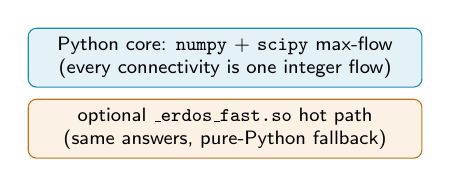
\begin{tikzpicture}[box/.style={rounded corners=3pt,minimum width=5.0cm,
        minimum height=0.72cm,font=\scriptsize,align=center}]
      \node[box,fill=KULblauw1!12,draw=KULblauw1] (p)
        {Python core: \texttt{numpy} + \texttt{scipy} max-flow\\(every connectivity is one integer flow)};
      \node[box,fill=vertexorange!12,draw=vertexorange!85!black,below=4pt of p] (c)
        {optional \texttt{\_erdos\_fast.so} hot path\\(same answers, pure-Python fallback)};
    \end{tikzpicture}\\[8pt]
    \footnotesize Measured speedups:
    \begin{itemize}\itemsep1pt\small
      \item dense max-flow \;$\approx 2\times$
      \item connectivity test \;$2.2\times$
      \item canonical form \;$\mathbf{147\times}$
    \end{itemize}
  \end{column}
\end{columns}

\vspace{0.3cm}
{\scriptsize\color{black!60}Annealing stays the default (its restarts parallelise trivially);
tabu is the sharper tool past the certified range.}
\end{frame}

% ----------------------------------------------------------------------------
% S11  RESULTS ON THE DIRECTED FRONTIER
% ----------------------------------------------------------------------------
\begin{frame}{Results on the directed frontier}
\begin{columns}[c,onlytextwidth]
  \begin{column}{0.54\textwidth}\centering
    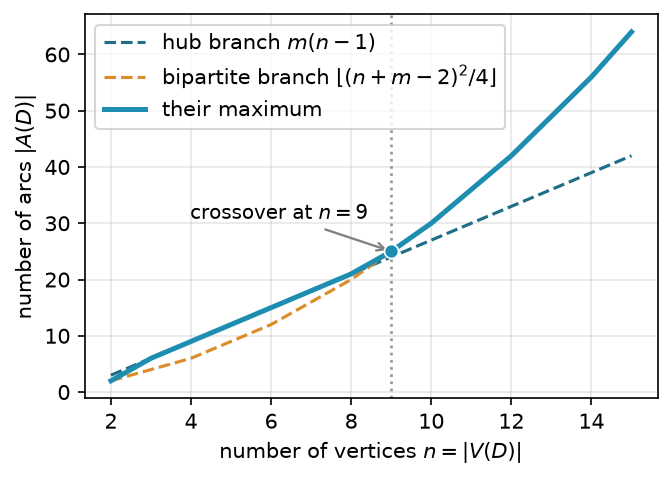
\includegraphics[width=\linewidth]{directed_crossover.png}\\[2pt]
    {\scriptsize\color{black!60}Two competing constructions at $m=3$. The linear hub leads early,
    the quadratic augmented-bipartite family overtakes near $n=9$.}
  \end{column}
  \begin{column}{0.44\textwidth}\small
    {\bfseries Two genuine advances:}\\[6pt]
    \chip{stProved}{solved} {\bfseries Hypergraph vertex problem}\\
    settled for all $r$ and all $n$ at $m\le 3$:
    \[k_m^{(r)}(n)=\floor{\tfrac{(m-1)(n-1)}{r-1}},\]
    via a new rank bound on incidence graphs.\\[8pt]
    \chip{stMachine}{reduced} {\bfseries Directed multigraph, $m=3$}\\
    the whole infinite family collapses to {\bfseries two finite checks} on
    $7$ vertices ($L_3^{\mathrm{dir}}(7)=24$ and its extremisers).
  \end{column}
\end{columns}
\end{frame}

% ----------------------------------------------------------------------------
% S12  THE WHOLE LANDSCAPE
% ----------------------------------------------------------------------------
\begin{frame}{The whole landscape}
\centering\renewcommand{\arraystretch}{1.12}\scriptsize
\begin{tabular}{@{}lll l@{}}
  \toprule
  Separation & Model & Value & Status \\
  \midrule
  \multicolumn{4}{@{}l}{\color{KULblauw3b}\bfseries Undirected}\\
  edge   & simple & $\floor{m(n-1)/2}$ & {\color{stProved}proved (Mader)}\\
  edge   & multi  & $(m-1)(n-1)$ & {\color{stProved}proved}\\
  edge   & hyper  & $\floor{(m-1)(n-1)/(r-1)}$ & {\color{stProved}proved (Gomory-Hu)}\\
  vertex & simple & $\floor{m(n-1)/2}$ \;($m\le4$),\; $\floor{8n/3}-3$ \;($m{=}5$) & {\color{stConj}cited,} {\color{stOpen}open $m\ge6$}\\
  vertex & multi  & parallel edges do not help & {\color{stProved}proved}\\
  vertex & hyper  & $\floor{(m-1)(n-1)/(r-1)}$ \;($m\le3$) & {\color{stProved}proved $m\le3$,} {\color{stOpen}open $m\ge4$}\\
  \midrule
  \multicolumn{4}{@{}l}{\color{KULblauw3b}\bfseries Directed}\\
  arc    & simple & $\max(2(n-1),\floor{n^2/4})$ \;($m{=}2$) & {\color{stProved}proved,} {\color{stConj}conj.\ $m\ge3$}\\
  arc    & multi  & $(m-1)\max(2(n-1),\floor{n^2/4})$ & {\color{stMachine}proved $n\le6$,} {\color{stConj}cond.\ $m{=}3$}\\
  arc    & hyper  & quadratic in $n$, exact value open & {\color{stOpen}lower bound}\\
  vertex & simple & $\max(2(n-1),\floor{n^2/4})$ \;($m{=}2$) & {\color{stProved}proved,} {\color{stConj}conj.\ $m\ge3$}\\
  vertex & multi  & reduces to simple digraph & {\color{stProved}proved}\\
  vertex & hyper  & quadratic in $n$, exact value open & {\color{stOpen}lower bound}\\
  \bottomrule
\end{tabular}

\vspace{0.15cm}
{\scriptsize \chip{stProved}{proved}\; \chip{stMachine}{certified}\;
\chip{stConj}{conjecture}\; \chip{stOpen}{open}}
\end{frame}

% ----------------------------------------------------------------------------
% S13  FUTURE AND CONCLUSION
% ----------------------------------------------------------------------------
\begin{frame}{What is left, and why it matters}
\begin{columns}[t,onlytextwidth]
  \begin{column}{0.55\textwidth}\small
    {\bfseries\color{KULblauw1}Open problems}
    \begin{itemize}\itemsep4pt
      \item {\bfseries Backward-arc lemma.} Proving an extremal non-hub digraph has no arc from
            $B$ to $A$ turns the directed conjecture into a theorem for all $m\ge3$.
      \item {\bfseries Two finite $n=7$ checks} close the directed multigraph problem at $m=3$.
            Memory-safe today, runtime-limited. Gurobi or the cluster would finish them.
      \item {\bfseries Vertex-disjoint $m\ge6$}, open since 1974.
      \item {\bfseries Hypergraph vertex $m\ge4$}, needing a 4-connectivity decomposition.
    \end{itemize}
  \end{column}
  \begin{column}{0.43\textwidth}\small
    {\bfseries\color{KULblauw1}The contribution}
    \begin{itemize}\itemsep4pt
      \item one representation for all twelve variants
      \item one exact connectivity checker
      \item one certifier for small-case upper bounds
      \item one cooled search for constructions
    \end{itemize}
    \vspace{0.5cm}
    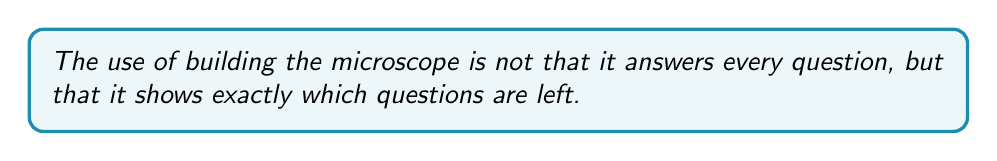
\begin{tikzpicture}\node[draw=KULblauw1,line width=1.2pt,rounded corners=5pt,
        fill=KULblauw1!8,inner sep=8pt,text width=\linewidth-22pt]
      {\itshape The use of building the microscope is not that it answers every question, but
       that it shows exactly which questions are left.};\end{tikzpicture}
  \end{column}
\end{columns}
\end{frame}

% ----------------------------------------------------------------------------
% CLOSING
% ----------------------------------------------------------------------------
\begin{frame}[plain]
\centering
\vspace{1.6cm}
{\color{KULblauw3b}\fontsize{30}{34}\selectfont\bfseries Thank you}\\[10pt]
{\large\color{black!70}Questions?}\\[18pt]
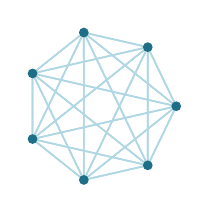
\begin{tikzpicture}[scale=0.8]
  \foreach \i in {0,...,6}{\coordinate (q\i) at ({51.43*\i}:1.2);}
  \foreach \i in {0,...,6}{\foreach \j in {0,...,6}{\draw[KULblauw1!35,line width=0.6pt] (q\i)--(q\j);}}
  \foreach \i in {0,...,6}{\fill[KULblauw3b] (q\i) circle (2.2pt);}
\end{tikzpicture}\\[10pt]
{\small\color{black!55}Backup slides follow: a deep dive into each variant.}
\end{frame}

% ============================================================================
%  BACKUP SLIDES  (for the question round)
% ============================================================================
\begin{frame}[plain]
\centering\vspace{2.2cm}
{\color{KULblauw3a}\Large BACKUP SLIDES}\\[8pt]
{\color{black!60}Dive deeper into any single variant.}
\end{frame}

% --- B1: directed arc conjecture ---
\begin{frame}{Backup: the directed arc conjecture}
\small
At $m=2$ the value is proved: $\ell_2^{\mathrm{dir}}(n)=\max(2(n-1),\floor{n^2/4})$, by an induction
deleting a minimum-degree vertex. The linear branch is the bidirected hub, the quadratic branch the
one-directional bipartite digraph, tying at $n=7$.

\vspace{0.3cm}
\begin{columns}[c,onlytextwidth]
  \begin{column}{0.5\textwidth}\centering
    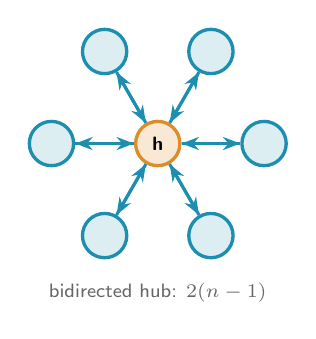
\begin{tikzpicture}[scale=0.9]
      \node[smallvertex,fill=vertexorange!20,draw=vertexorange] (h) at (0,0) {h};
      \foreach \a in {0,60,120,180,240,300}{\node[smallvertex] (v\a) at (\a:1.5){};}
      \foreach \a in {0,60,120,180,240,300}{\draw[arc] (h)--(v\a); \draw[arc] (v\a)--(h);}
      \node[font=\scriptsize\color{black!60}] at (0,-2.1) {bidirected hub: $2(n-1)$};
    \end{tikzpicture}
  \end{column}
  \begin{column}{0.5\textwidth}\centering
    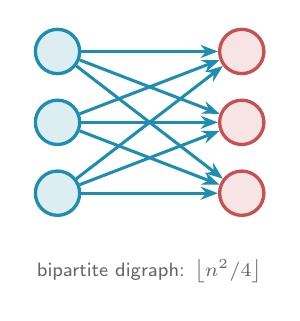
\begin{tikzpicture}[scale=0.9]
      \foreach \i in {0,1,2}{\node[smallvertex,fill=KULblauw1!15] (a\i) at (-1.3,1-\i){};}
      \foreach \i in {0,1,2}{\node[smallvertex,fill=vertexred!15,draw=vertexred] (b\i) at (1.3,1-\i){};}
      \foreach \i in {0,1,2}{\foreach \j in {0,1,2}{\draw[arc] (a\i)--(b\j);}}
      \node[font=\scriptsize\color{black!60}] at (0,-2.1) {bipartite digraph: $\floor{n^2/4}$};
    \end{tikzpicture}
  \end{column}
\end{columns}

\vspace{0.2cm}
For $m\ge3$ the conjecture adds the augmented-bipartite family. The missing piece is the
{\bfseries backward-arc lemma} for the matching upper bound.
\end{frame}

% --- B2: hypergraph vertex / incidence rank ---
\begin{frame}{Backup: the hypergraph vertex problem}
\small
Routes in an $r$-uniform hypergraph are {\bfseries Berge paths}, alternating vertices and hyperedges.
A single hyperedge serves only one route, so two Berge routes are disjoint when they share no hyperedge.

\vspace{0.3cm}
\begin{columns}[c,onlytextwidth]
  \begin{column}{0.45\textwidth}\centering
    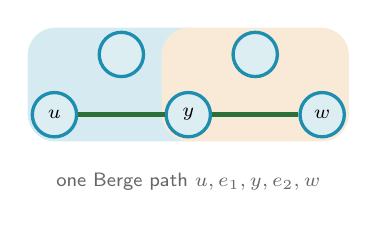
\begin{tikzpicture}[scale=0.85]
      \node[smallvertex] (u) at (-2,0) {$u$};
      \node[smallvertex] (x) at (-1,0.9){};
      \node[smallvertex] (y) at (0,0)  {$y$};
      \node[smallvertex] (z) at (1,0.9){};
      \node[smallvertex] (w) at (2,0)  {$w$};
      \begin{pgfonlayer}{background}
        \fill[KULblauw1!18,rounded corners=10pt] (-2.4,-0.4) rectangle (0.4,1.3);
        \fill[vertexorange!18,rounded corners=10pt] (-0.4,-0.4) rectangle (2.4,1.3);
      \end{pgfonlayer}
      \draw[line width=2pt,vertexgreen!70!black] (u)--(y)--(w);
      \node[font=\scriptsize\color{black!60}] at (0,-1.0) {one Berge path $u,e_1,y,e_2,w$};
    \end{tikzpicture}
  \end{column}
  \begin{column}{0.53\textwidth}
    {\bfseries Result.} For $m\le 3$, every uniformity $r$, all $n$:
    \[k_m^{(r)}(n)=\floor{\tfrac{(m-1)(n-1)}{r-1}}=\ell_m^{(r)}(n).\]
    The $m=3$ proof rests on a {\bfseries rank bound for incidence graphs},
    derived through Tutte's triconnected (SPQR) decomposition, valid exactly where
    $\kappa\le2$.\\[6pt]
    {\bfseries Open at $m\ge4$:} it would need a 4-connectivity analogue of that decomposition.
    No early counterexample: $k_4^{(3)}(5)=6$ machine-checked.
  \end{column}
\end{columns}
\end{frame}

% --- B3: the n=7 reduction ---
\begin{frame}{Backup: collapsing an infinite family to two checks}
\small
The directed multigraph problem at $m=3$ is reduced, not assumed, to a finite computation.

\vspace{0.4cm}
\centering
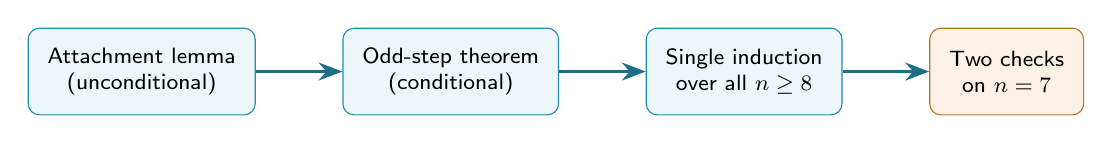
\begin{tikzpicture}[node distance=0.6cm,
   stp/.style={rounded corners=4pt,draw=KULblauw1,fill=KULblauw1!8,
               font=\footnotesize,align=center,inner sep=7pt,minimum height=1.1cm},
   ar/.style={-{Stealth[length=3mm]},line width=1.4pt,KULblauw3b}]
  \node[stp] (a) {Attachment lemma\\(unconditional)};
  \node[stp,right=1.1cm of a] (b) {Odd-step theorem\\(conditional)};
  \node[stp,right=1.1cm of b] (c) {Single induction\\over all $n\ge8$};
  \node[stp,right=1.1cm of c,fill=vertexorange!12,draw=vertexorange!85!black] (d)
    {Two checks\\on $n=7$};
  \draw[ar] (a)--(b); \draw[ar] (b)--(c); \draw[ar] (c)--(d);
\end{tikzpicture}

\vspace{0.5cm}
The two remaining facts, on multigraphs with multiplicities in $\{0,1,2\}$:
\begin{itemize}\itemsep3pt\small
  \item[(a)] $L_3^{\mathrm{dir}}(7)=24$;
  \item[(b)] the only $24$-arc extremisers (max degree $\le 8$) are
        $2B_{3,4}$, $2B_{4,3}$, and the doubled bidirected path $P_7$.
\end{itemize}
\vspace{2pt}
{\scriptsize\color{black!60}This bypasses the unproved minimum-degree conjecture entirely. The wall
is now runtime, not structure.}
\end{frame}

% --- B4: Gomory-Hu storage ---
\begin{frame}{Backup: how connectivity is stored}
\small
A {\bfseries Gomory-Hu tree} is a weighted tree on the same vertices in which $\lambda_G(u,v)$
is the lightest edge on the tree path from $u$ to $v$. All $\binom{n}{2}$ connectivities live in
$n-1$ numbers, and $\lmax_G$ is simply the heaviest tree edge.

\vspace{0.3cm}
\centering
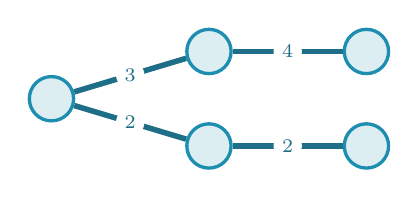
\begin{tikzpicture}[scale=1.0]
  \node[smallvertex] (a) at (0,0) {};
  \node[smallvertex] (b) at (2,0.6){};
  \node[smallvertex] (c) at (2,-0.6){};
  \node[smallvertex] (d) at (4,0.6){};
  \node[smallvertex] (e) at (4,-0.6){};
  \draw[treeedge,line width=2pt] (a)--(b) node[treeweight,midway]{$3$};
  \draw[treeedge,line width=2pt] (a)--(c) node[treeweight,midway]{$2$};
  \draw[treeedge,line width=2pt] (b)--(d) node[treeweight,midway]{$4$};
  \draw[treeedge,line width=2pt] (c)--(e) node[treeweight,midway]{$2$};
\end{tikzpicture}

\vspace{0.3cm}
This is exactly the structure the checker and the Mader proof both lean on: store the whole
connectivity profile cheaply, read off the binding pair instantly.
\end{frame}

% --- B5: values cheat-sheet ---
\begin{frame}{Backup: values at a glance}
\small
\centering
\begin{tabular}{@{}ll@{}}
  \toprule
  Object & Extremal value \\
  \midrule
  simple undirected edge, $\ell_m(n)$ & $\floor{m(n-1)/2}$ \\
  multigraph edge, $L_m(n)$ & $(m-1)(n-1)$ \\
  hypergraph edge, $\ell_m^{(r)}(n)$ & $\floor{(m-1)(n-1)/(r-1)}$ \\
  simple vertex, $k_m(n)$ \;($m\le4$) & $\floor{m(n-1)/2}$ \\
  simple vertex, $k_5(n)$ & $\floor{8n/3}-3$ \\
  directed arc, $m=2$ & $\max(2(n-1),\floor{n^2/4})$ \\
  directed multigraph arc & $(m-1)\max(2(n-1),\floor{n^2/4})$ \\
  hypergraph vertex, $m\le3$ & $\floor{(m-1)(n-1)/(r-1)}$ \\
  random-graph threshold & $p^\ast=m/n$ \\
  \bottomrule
\end{tabular}

\vspace{0.4cm}
{\scriptsize\color{black!60}$n$ vertices, threshold $m$ (no pair gets $m$ routes), uniformity $r$.}
\end{frame}

\end{document}
